\chapter{Elvégzett munka}


\section{Koncepció}
Állapottérképek formális verifikációjának támogatása MagicDraw-ban, egy plug-in fejlesztésével lett megvalósítva. A plug-in függ a Viatra For MagicDraw-tól, ami lehetővé teszi modellek transzformációját Viatra segítségével aminek a 2.0.1-es verziója van használva. A plug-in legfontosabb funkciója MagicDraw modellek Gamma modellekké való transzformációja. A letranszformált már Gamma nyelvű modelleket az keretrendszer kezelni tudja, a verifikáció elvégzéséhez az eszköznek csak egyes részei szükségesek (\ref{fig:used-gamma} ábra). A plug-in MagicDrawToGammának lett elnevezve.

\begin{figure}[!ht]
	\centering
	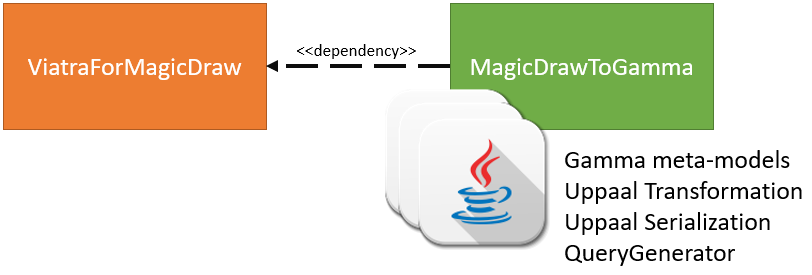
\includegraphics[keepaspectratio, width=120mm]{figures/plan.png}
	\caption{Architektúra koncepció}
	\label{fig:used-gamma}
\end{figure}

\section{Fejlesztőkörnyezet}
 A fejlesztés megkezdéséhez szükséges volt összeállítani egy olyan fejlesztőkörnyezetet amivel hatékonyan lehet plug-int fejleszteni. MagicDraw biztosít egy ún. skeletont Eclipsehez és IntelliJhez is plug-in fejlesztéséhez, de a fejlesztés nem ezek segítségével hanem az IncQueryLabs által készített skeleton felhasználásával valósult meg. Ez már elő volt készítve V4MD használatához.
 
A skeleton egy Eclipse project, viszont Gradlet használ a projekt fordításához és a dependenciák kezeléséhez, ez sokszor inkonzisztenciákhoz vezetett, az egyik legnagyobb probléma a Viatra Querik generálása amit Gradleel nem csak Eclipsel lehet generálni. A kódbázis egy része nem Javában hanem Xtendben íródott, a Viatra modell transzformációk implementálása ezzel a nyelvvel egyszerűbb, azok az osztályok melyeknél nem volt indokolt, jellemzően a MagicDraw felhasználói felületeinél, azok Java 8-ban lettek implementálva.

A dolgozat elkészítése idején a MagicDraw 19-es verziója is elérhető volt a plug-in azonban még nem ehhez, hanem a 18.5-ös verziójához készült. A kódbázis azonban kompatibilis lehet még az újabb verziókkal is, amennyiben az állapottérképeket érintő meta-modellek nem változnak.

Gamma a verifikációt Uppaal segítségével végzi el, ehhez előállít egy leírást a rendszerről és egy queryt ami a rendszerrel szemben támasztott követelményeket írja le. Utóbbi megírásához biztosít egy UI elemet amivel a felhasználó az Uppaal ismerete nélkül is képes a követelmények definiálására. Ez a funkció teljesen át lett emelve Gammából módosított implementációval a MagicDrawToGammába. A Gamma az Uppaalra az operációs rendszeren keresztül hív át, ezért az Uppaalt külön kell telepíteni és konfigurálni.

\section{MagicDraw - Gamma transzformáció}

A MagicDraw - Gamma transzfromációt egy menü elemmel lehet elindítani, ehhez szükséges, hogy a projekthez hozzá legyen rendelve egy külső könyvtár (Gamma Workspace) ami a leképzett és perzisztensen eltárolandó modellek helyét jelöli. A hozzárendelt könyvtár abszolút elérését String formában a projekt tárolja, emiatt nem migrálható, sem pedig maga a Gamma Workspace. Továbbá a könyvtár karbantartása ebben a verzióban még a felhasználó felelőssége, ugyanis a plug-in nem töröl a könyvtárból csak hozzáad és módosít, ennek akkor van jelentősége, ha a modell le lett képezve, ezután egy állapottérkép el lett távolítva utána újra le lett képezve. Ebben az esetben a régebben leképzett Gamma állapottérképek is megmaradnak.

\subparagraph{Előkészítés:}

A plugin a transzformáió elején létrehoz egy ResourceSet-et, amibe készít egy Resource-t a Gamma Workpace gyökerébe .traces.md2g néven, továbbá egy Resource-t interfaces.gms néven. Az előbbi Resource egy segédstruktúrát tartalmaz ami a leképzett elemek visszakereshetőségéül szolgál (ld. \refstruc{sec:trace_model}), utóbbi pedig a modellben definiált interfaceket tárolja.

Az eszköz ezután Viatra Queryk segítségével megkeresi az állapotgépeket a MagicDrawban és végig iterál rajtuk. Minden állapottérképen kigyűjti az éleken használt Signal Eventeket és létrehoz a Signaléval azonos néven egy Eventet, a Gamma meta-modelljének megfelelően. A létrehozott eventek egy Interfacen kerülnek definiálásra aminek a neve megegyezik az állapottérképével. Az interface ezután belekerül az interfaceket tároló Resourceba. eventek iránya INOUT ez lehetővé teszi azt is, hogy az állapotgép magának küldjön eseményt.

A leképzett állapottérképek külön Resourceokba kerülnek amik a Gamma Workspace-ben egy külön az állapottérkép nevével megegyező könyvtárba kerülnek, ugyan ezen a néven .gsm kiterjesztéssel (\ref{fig:filestructure}-es ábra). (A Resource gyökere nem egy StatechartDefinition, hanem egy Package, ennek a neve szintén megegyezik az állapottérkép nevével)

\begin{figure}[!ht]
	\centering
	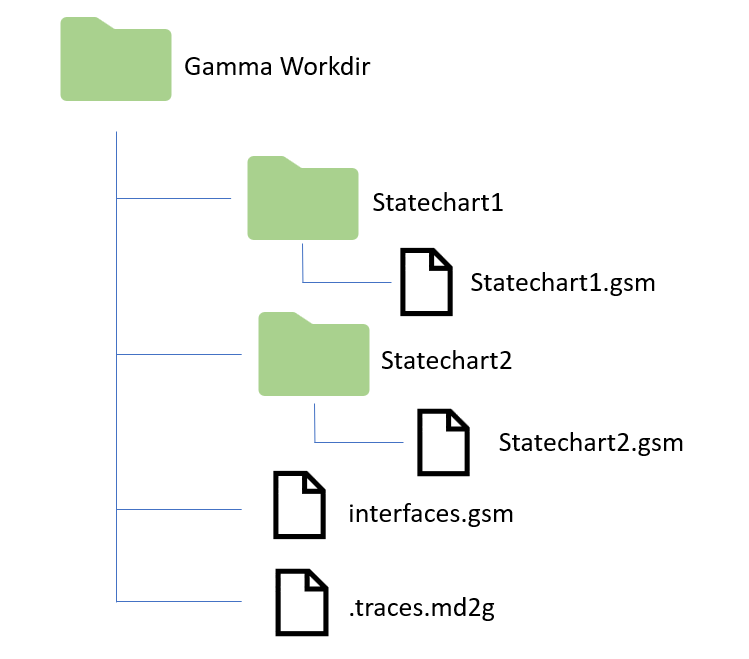
\includegraphics[keepaspectratio, width=90mm]{figures/filestructure.png}
	\caption{Létrehozott fájlstruktúra}
	\label{fig:filestructure}
\end{figure}

\subparagraph{Alap struktúra kialakítása:}

Az előző lépések során azok az elemek állnak elő, melyek a modellek gyökér elemeiként fognak szolgálni. A következő lépés létrehozni az állapottérképek egy belső, alap struktúráját, amit az állapotok ás állapotátmenetek határoznak meg. Ehhez a plug-in a Viatra Batch Transformationját használta fel. A Viatra for MagicDraw projekt megnyitásakor készít egy ViatraQueryEngine-t aminek a Scope-ja a megnyitott modellre terjed ki. A transzformációs szabályok regisztrálása ezen az engine-en történik, létrejön azonban még egy aminek a Scopje magában foglalja az első lépésben lérehozott Resourceokat és a MagicDraw modellt is. A készülő modellben történő keresések, és a visszakövetések ezzel az engine-el történnek. Alap struktúra kialakításának lépcsői:

\begin{enumerate}
	\item Fő régiók leképzése (olyan régió aminek a szülője állapotgép).
	\label{enum:elso}
	\item Régiókban található állapotok leképzése.
	\label{enum:masodik}
	\item Állapotokban található régiók leképzése.
	\label{enum:harmadik}
\end{enumerate}


A 2. lépésben a Trace Modell alapján megkeressük a már leképzett régiót a Gamma Modellben és beletesszük az újonnan létrehozott és a MagicDraw modellnek megfelelően elnevezett állapotot, ha a régió még nincs leképezve akkor létrejön, és abba kerül bele az állapotot. Ez a lépés olyan részgráfokat is eredményezhet amikbe nem vezet út a gyökér elemekből. Ennek kiküszöbölése a 3. lépés ami, ugyan ezt a műveletet hajtja végre csak a másik irányból, tehát az állapotok párjait keressük meg, amikbe régiókat helyezünk el, ezek a régiók már létezhetnek ilyenkor nem új régió jön létre hanem a már meglévő kerül az állapotba. A működés során a MagicDraw modell jól formáltsága kihasznált és elvárt, továbbá az is ki van használva, hogy régió csak Stateben és Állapotgépben lehet. A régiókat tartalmazó állapotok kompozit és ortogonális állapotnak tekintendők.

A tartalmazási gráf összefüggővé válását \aref{fig:state-transformation} ábra szemlélteti.

\begin{figure}[!h]
Az irányított nyilak tartalmazást jelölnek, a bekeretezett téglalap StatechartDefinition, a szagatott vonallal körbevett Region és a körök Statek.

\centering
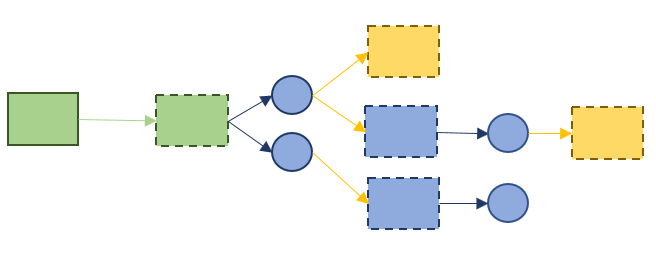
\includegraphics[keepaspectratio, width=100mm]{figures/transformation.png}
\caption{Állapotok és régiók leképzésének menete, \ref{enum:elso}. lépcső: zöld, \ref{enum:masodik}. lépcső: kék, \ref{enum:harmadik}. lépcső: sárga}
\label{fig:state-transformation}
\end{figure}


\subparagraph{Pszeudoállapotok átalakítása:}
Az állapotátmenetek leképzése előtt a pszeudoállapotok kerülnek leképzésre, ezen a ponton már létezik minden régió amit tartalmazhatja őket. A leképzés legtöbb esetben támogatott viszont, egyes elemek tartalmazása esetén nem lehet a verifikációt végrehajtani. Az elemeket és párjaikat \aref{table:pseudo} táblázat mutatja.

\begin{table}[ht]
	\footnotesize
	\centering
	\begin{tabular}{ l c c }
		MagicDraw & Gamma & verifikálható \\ \hline
		InitialState & InitialState & igen \\
		Chioce & Choice & igen \\
		Junction & Merge & nem \\
		Fork & Fork & nem \\
		Join & Join & nem \\
		TerminalState & nincs & - \\
		Conn. PointReference & nincs & - \\
		EntryPoint & nincs & - \\
		ExitPoint & nincs & -
		
	\end{tabular}
	\caption{Pszeudoállapotok párosítása.}
	\label{table:pseudo}
\end{table}

\subparagraph{Állapotátmenetek leképzése:} A következő lépés az állapotátmenetek átalakítása. Ezen a ponton már az összes olyan elem leképzésre került, amely az állapotátmenetek kezdő, vagy végpontjaként szolgálhat. Egy MagicDraw modellben az állapotátmenetek régiók tartalmazzák, szemben Gammával, ahol a StatechartDefinitionban közvetlen gyerekei. A tartalmazó-tartalmazott, Statemahcine - Tranisiton párok megkeresése a következő patternekkel történik.
\begin{lstlisting}
pattern RegionsInRegion(container: Region, region: Region){
	Region.subvertex(container, vertex);
	State.region(vertex, region);
}

pattern RegionsInStatemachine(stateMachine: StateMachine, subregion: Region){
	find MainRegions(stateMachine, subregion);
} or {
	find RegionsInRegion+(region, subregion);
	StateMachine.region(stateMachine, region);
}

pattern TranisitonsInStateMachine(stateMachine: StateMachine, transition: Transition){
	find RegionsInStatemachine(stateMachine, region);
	Region.transition(region, transition);
}
\end{lstlisting}

A StateMachine Gamma modellbeli párját a Trace modell segítségével lehet megtalálni és hozzáadni a megfelelő állapotátmenetet.

Az átmenetek leképzése után már elérhetőséget lehet is vizsgálni.

\subparagraph{Triggerek leképzése:}

\subparagraph{Guardok leképzése:}

\subparagraph{Akciók leképzése:}

\subsection{Trace Model}

\label{sec:trace_model}
